\SourceLeaf{318}
am leichtesten missverstanden werden kann. Drittens hätte auch hier ausdrücklich
in Beziehung auf das Beispiel eine literirte Figur beigefügt werden müssen. Und
viertens glaube ich sogar einen Schreibfehler begangen und anstatt
$60^0+60^0=120^0$ geschrieben zu haben $30^0+30^0=60^0$. Wollte ich nun diese
3 oder 4 Punkte alle und ganz aufklären, so würde dazu ein längerer Brief
nöthig sein, als ich heute schreiben kann. Einstweilen ignoriren Sie also das
Beispiel mit dem gleichseitigen Dreieck ganz (was ich übrigens, wenn es der
Mühe werth scheinen sollte, zu einer andern Zeit zu erklären gern erbötig
bin). Dagegen will ich heute zu weiterer Verständigung über das allgemeine
Theorem das Nöthige beifügen.

Vor allem aber muss ich, um jedes Missverständniss darüber auszuschliessen,
ausdrücklich bemerken, was die Data des \textsc{Pothenot}schen Problems nothwendig
enthalten müssen:

1) müssen die drei gegebenen [Punkte, wenigstens ihrer gegenseitigen \textls[120]{Lage}
nach, vollkommen bestimmt sein, so dass über das Rechts- oder Linksliegen
keine Zweideutigkeit ist. Es ist also z.\,B. nicht zureichend, die Grösse der
Winkel zu kennen, sondern auch ihre \textls[120]{Lage}; also z.\,B. nicht bloss $A=45^0$,
$B=45^0$, $C=90^0$, weil so das Dreieck

\begin{center}\begin{tabular}{c@{\quad}c@{\quad}c@{\quad}l}\resizebox{1.65cm}{!}{%
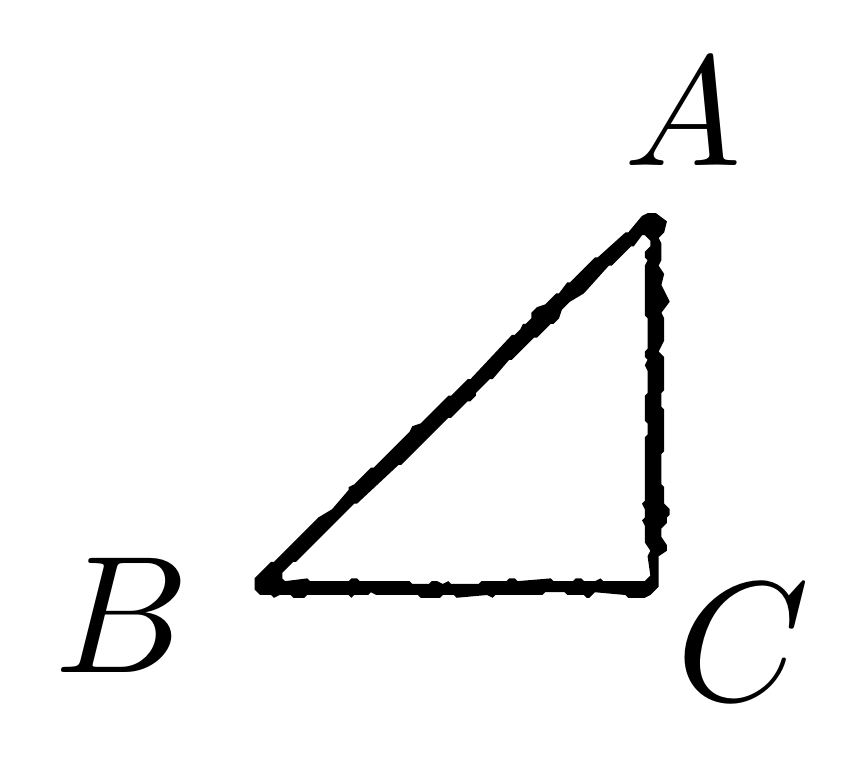
\begin{tikzpicture}[x=1pt,y=-1pt]
\path[use as bounding box] (0,0) rectangle (290,255);
\path[fill=black,draw=none,even odd rule]
(231,70) -- (227,67) -- (224,67) -- (222,68) -- (217,74) -- (216,74) -- (206,83) -- (205,83) -- (196,92) -- (195,92) -- (192,96) -- (191,96) -- (187,100) -- (184,101) -- (182,103) -- (182,105) -- (180,107) -- (179,107) -- (178,109) -- (176,111) -- (175,111) -- (160,127) -- (159,127) -- (153,133) -- (152,133) -- (142,143) -- (139,144) -- (138,146) -- (125,159) -- (124,159) -- (118,165) -- (116,166) -- (116,167) -- (110,174) -- (105,177) -- (89,193) -- (88,193) -- (82,199) -- (82,203) -- (84,205) -- (88,205) -- (89,206) -- (91,205) -- (95,205) -- (96,206) -- (100,206) -- (101,205) -- (116,205) -- (117,206) -- (118,205) -- (123,205) -- (124,204) -- (126,205) -- (141,205) -- (142,206) -- (149,206) -- (150,205) -- (154,205) -- (155,206) -- (166,205) -- (168,206) -- (169,205) -- (186,205) -- (187,204) -- (194,204) -- (195,205) -- (201,205) -- (202,206) -- (203,206) -- (205,204) -- (216,205) -- (217,206) -- (223,206) -- (225,205) -- (228,202) -- (228,191) -- (231,189) -- (231,187) -- (229,184) -- (229,181) -- (231,179) -- (231,177) -- (232,176) -- (232,174) -- (230,172) -- (230,166) -- (229,165) -- (229,154) -- (230,153) -- (230,138) -- (229,137) -- (229,132) -- (230,131) -- (230,119) -- (228,117) -- (230,113) -- (230,105) -- (229,103) -- (232,99) -- (229,93) -- (230,89) -- (228,86) -- (229,84) -- (229,78) -- (228,76) -- (230,74) -- cycle
(225,77) -- (225,79) -- (223,81) -- (223,83) -- (224,84) -- (223,86) -- (223,104) -- (224,105) -- (224,116) -- (223,117) -- (223,119) -- (224,120) -- (223,122) -- (224,124) -- (224,132) -- (223,133) -- (223,142) -- (224,143) -- (224,147) -- (223,148) -- (223,171) -- (222,172) -- (223,174) -- (223,177) -- (222,178) -- (223,180) -- (223,186) -- (225,189) -- (224,191) -- (225,198) -- (223,200) -- (208,200) -- (207,199) -- (205,200) -- (201,200) -- (200,199) -- (198,199) -- (197,200) -- (190,200) -- (189,199) -- (177,200) -- (176,199) -- (174,199) -- (173,200) -- (164,200) -- (163,201) -- (153,201) -- (152,200) -- (150,201) -- (148,200) -- (146,200) -- (145,201) -- (139,201) -- (138,200) -- (120,200) -- (119,199) -- (117,199) -- (116,200) -- (102,200) -- (101,199) -- (93,200) -- (92,199) -- (92,197) -- (96,193) -- (97,193) -- (118,172) -- (119,172) -- (134,158) -- (135,158) -- (152,141) -- (153,141) -- (159,135) -- (160,135) -- (162,133) -- (162,132) -- (167,127) -- (168,127) -- (174,120) -- (175,120) -- (183,112) -- (184,112) -- (189,107) -- (190,107) -- (192,105) -- (193,102) -- (196,99) -- (201,96) -- (210,86) -- (211,86) -- (218,79) -- (219,79) -- (222,75) -- (223,75) -- cycle;
\node[inner sep=0pt,font=\fontsize{10}{10}\selectfont] at (237.0,30.5) {\scalebox{5.643}{$A$}};
\node[inner sep=0pt,font=\fontsize{10}{10}\selectfont] at (34.0,212.5) {\scalebox{6.039}{$B$}};
\node[inner sep=0pt,font=\fontsize{10}{10}\selectfont] at (258.5,222.0) {\scalebox{6.138}{$C$}};
\end{tikzpicture}%
}
&nicht von&\resizebox{1.65cm}{!}{%
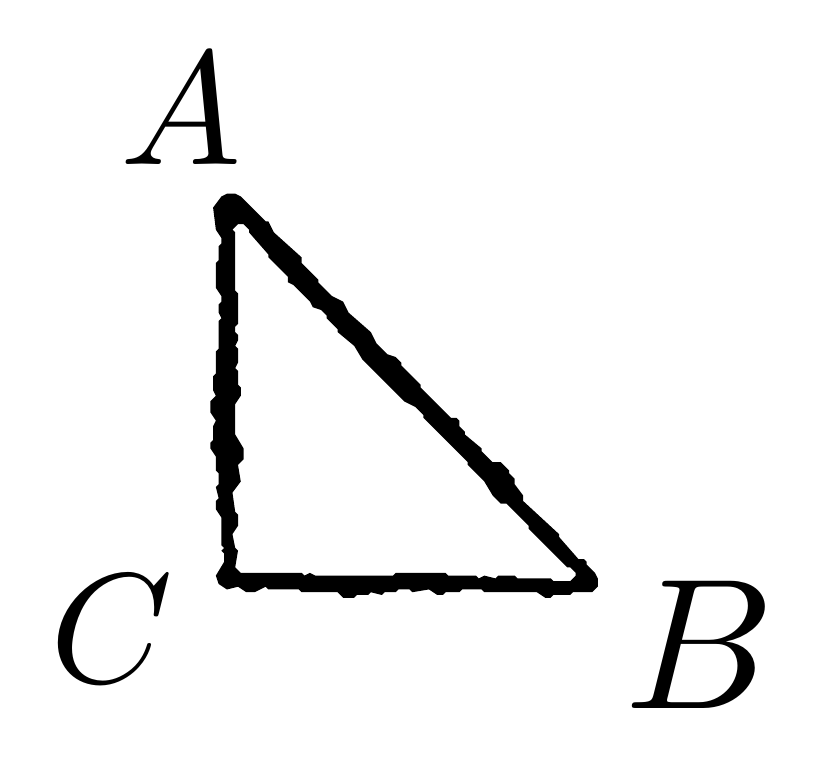
\begin{tikzpicture}[x=1pt,y=-1pt]
\path[use as bounding box] (0,0) rectangle (276,259);
\path[fill=black,draw=none,even odd rule]
(70,61) -- (67,65) -- (68,73) -- (70,76) -- (70,78) -- (69,79) -- (69,84) -- (68,85) -- (68,94) -- (70,97) -- (70,99) -- (69,100) -- (69,103) -- (70,105) -- (69,106) -- (69,116) -- (68,117) -- (68,125) -- (67,126) -- (67,131) -- (68,133) -- (66,135) -- (66,139) -- (68,142) -- (67,144) -- (67,149) -- (66,150) -- (66,152) -- (68,155) -- (68,160) -- (69,161) -- (69,165) -- (68,166) -- (69,170) -- (68,171) -- (68,174) -- (70,177) -- (70,187) -- (71,188) -- (70,189) -- (71,190) -- (71,193) -- (68,198) -- (69,201) -- (72,203) -- (76,202) -- (79,204) -- (82,204) -- (86,202) -- (87,203) -- (98,203) -- (99,204) -- (112,204) -- (114,206) -- (118,206) -- (119,205) -- (123,205) -- (124,204) -- (128,205) -- (129,204) -- (133,204) -- (134,203) -- (138,203) -- (139,204) -- (145,203) -- (148,205) -- (150,205) -- (151,204) -- (156,204) -- (157,203) -- (164,203) -- (165,204) -- (184,204) -- (187,206) -- (189,206) -- (190,205) -- (196,205) -- (197,204) -- (204,204) -- (206,202) -- (206,199) -- (205,197) -- (202,194) -- (202,193) -- (201,192) -- (199,192) -- (192,184) -- (192,183) -- (179,171) -- (179,169) -- (176,165) -- (176,163) -- (174,161) -- (174,160) -- (171,157) -- (168,157) -- (164,153) -- (164,152) -- (158,147) -- (158,146) -- (156,144) -- (156,142) -- (155,141) -- (153,141) -- (142,130) -- (142,129) -- (135,122) -- (135,121) -- (133,119) -- (130,118) -- (126,114) -- (124,110) -- (116,103) -- (114,99) -- (110,97) -- (105,92) -- (105,91) -- (99,85) -- (99,83) -- (89,74) -- (87,70) -- (86,70) -- (77,61) -- (75,60) -- (72,60) -- cycle
(76,71) -- (78,71) -- (80,73) -- (80,74) -- (87,82) -- (87,83) -- (94,90) -- (94,92) -- (96,93) -- (102,99) -- (103,101) -- (106,102) -- (108,104) -- (108,105) -- (112,109) -- (112,110) -- (118,115) -- (121,120) -- (136,135) -- (140,137) -- (143,140) -- (143,141) -- (159,157) -- (159,158) -- (165,164) -- (168,169) -- (171,172) -- (173,172) -- (181,180) -- (181,181) -- (195,195) -- (196,195) -- (198,197) -- (198,198) -- (196,200) -- (190,200) -- (189,199) -- (177,199) -- (176,198) -- (170,198) -- (169,199) -- (165,198) -- (163,199) -- (162,198) -- (152,198) -- (151,197) -- (133,197) -- (132,198) -- (104,198) -- (102,197) -- (100,198) -- (99,197) -- (77,197) -- (75,195) -- (76,189) -- (75,188) -- (74,183) -- (76,180) -- (76,176) -- (75,175) -- (74,168) -- (77,164) -- (76,158) -- (78,156) -- (78,152) -- (75,147) -- (75,136) -- (77,133) -- (77,130) -- (76,129) -- (76,124) -- (75,123) -- (76,121) -- (76,116) -- (75,115) -- (76,113) -- (76,111) -- (75,110) -- (75,108) -- (76,107) -- (76,96) -- (75,95) -- (75,74) -- (74,73) -- cycle;
\node[inner sep=0pt,font=\fontsize{10}{10}\selectfont] at (55.5,29.5) {\scalebox{5.841}{$A$}};
\node[inner sep=0pt,font=\fontsize{10}{10}\selectfont] at (30.5,217.5) {\scalebox{5.643}{$C$}};
\node[inner sep=0pt,font=\fontsize{10}{10}\selectfont] at (243.0,223.0) {\scalebox{6.732}{$B$}};
\end{tikzpicture}%
}
&unterschieden würde.\end{tabular}\end{center}

2) wird dieselbe vollständige Bestimmtheit für die Winkel an dem gesuchten
Punkte $X$ erfordert.

Es ist also z.\,B. nicht zureichend zu sagen, dass in $X$ der Winkel zwischen
$A$ und $B$ $40^0$, zwischen $B$ und $C$ $100^0$ sein soll, weil sonst

\begin{center}\resizebox{4.7cm}{!}{%
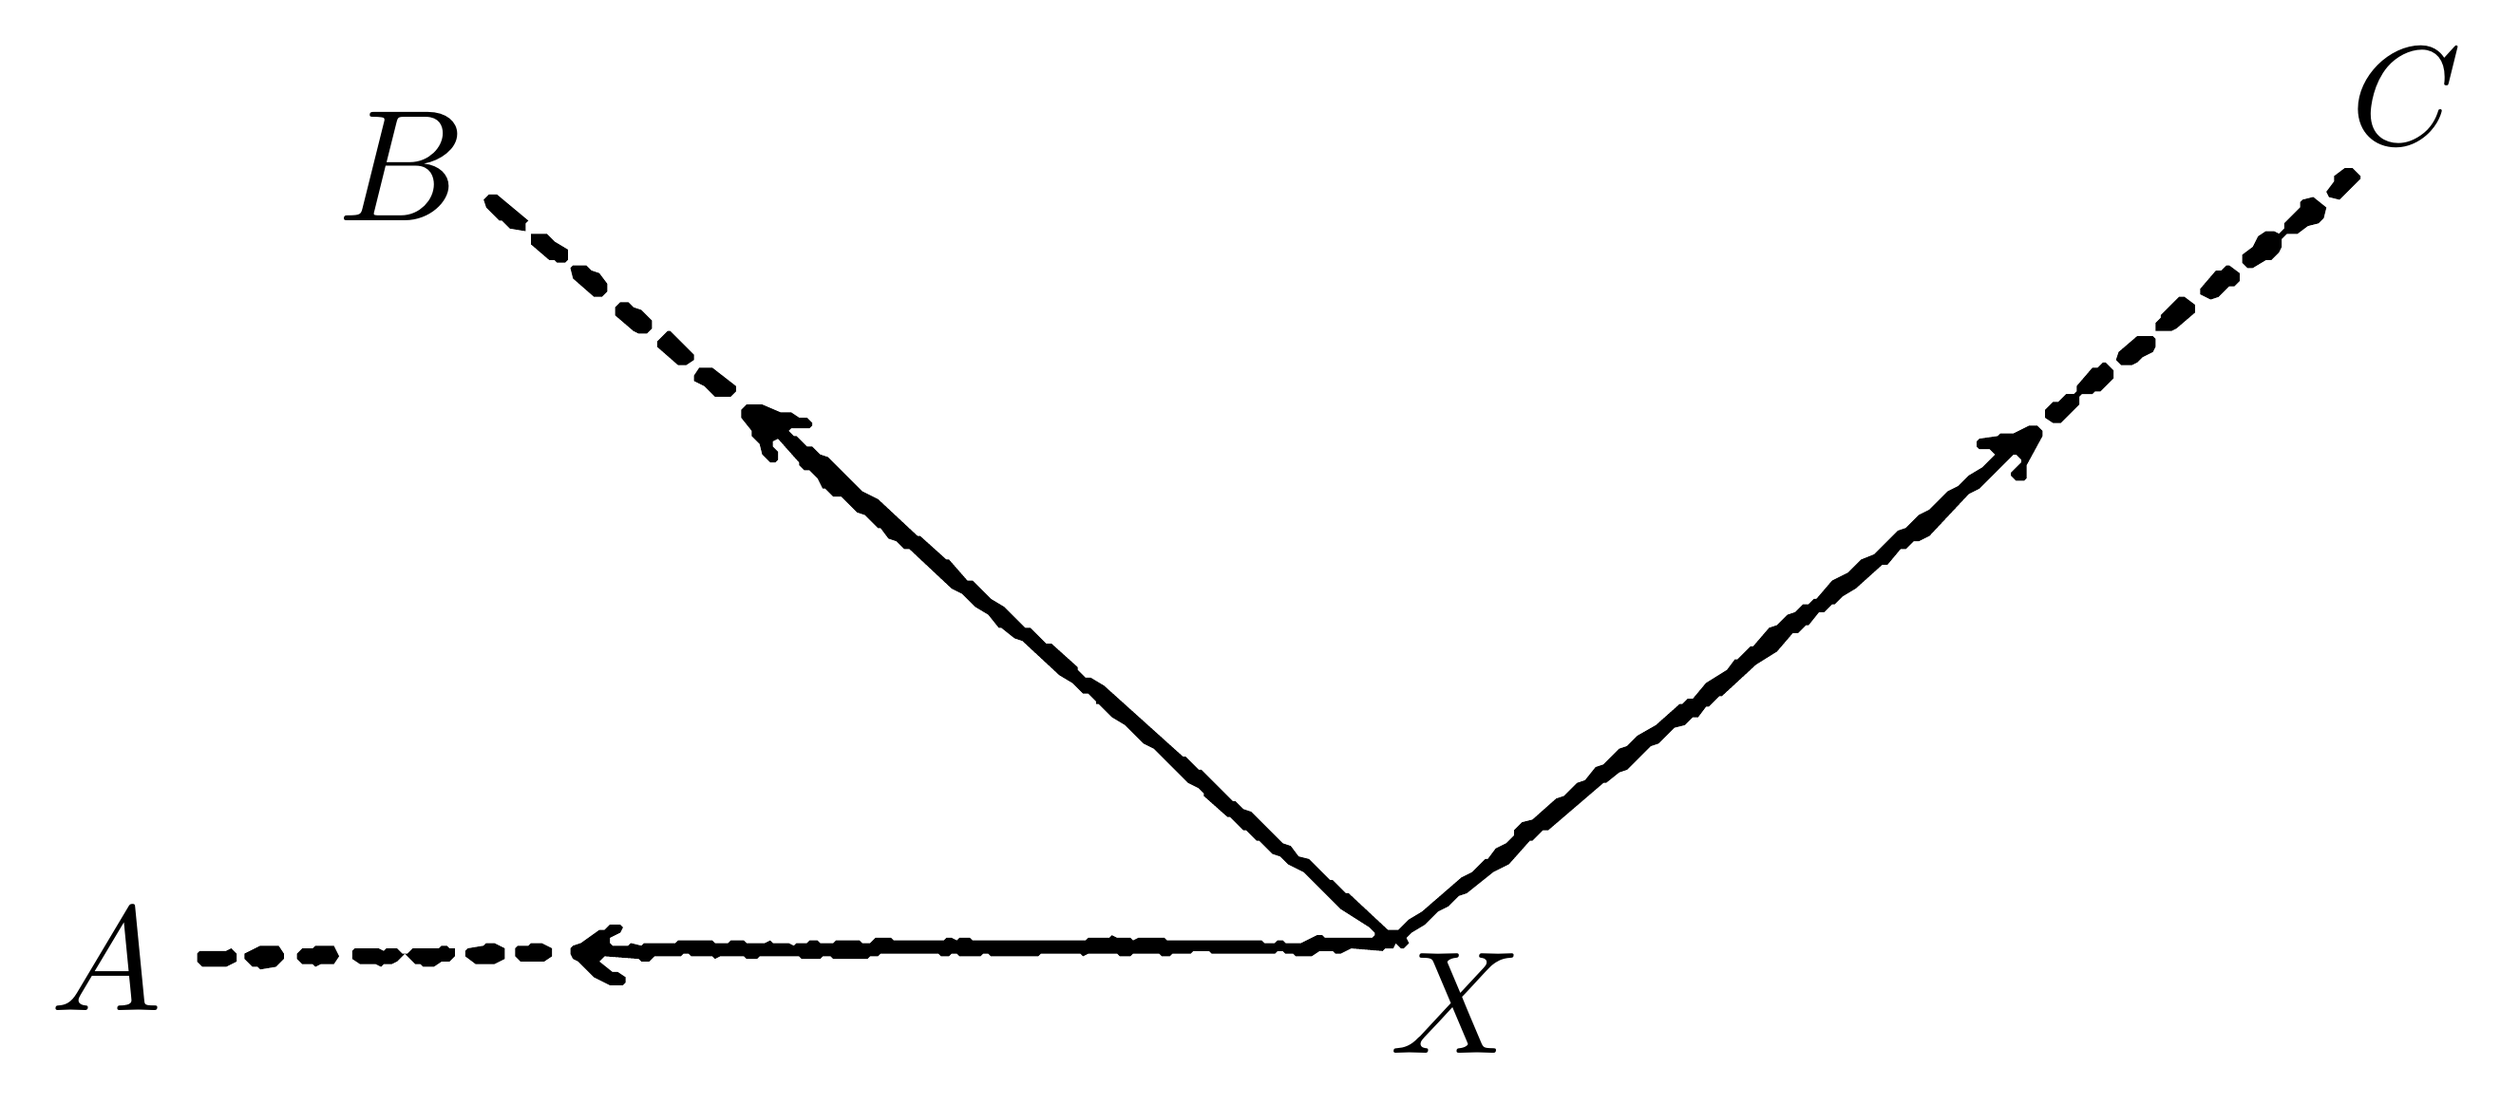
\begin{tikzpicture}[x=1pt,y=-1pt]
\path[use as bounding box] (0,0) rectangle (931,400);
\path[fill=black,draw=none,even odd rule]
(80,353) -- (78,351) -- (76,352) -- (66,352) -- (65,353) -- (65,356) -- (67,358) -- (76,358) -- (80,356) -- cycle
(163,351) -- (161,351) -- (160,350) -- (158,350) -- (157,351) -- (147,351) -- (145,353) -- (143,353) -- (141,351) -- (137,351) -- (136,352) -- (134,351) -- (125,351) -- (124,352) -- (124,355) -- (127,357) -- (133,357) -- (135,358) -- (136,357) -- (139,357) -- (141,356) -- (144,353) -- (148,357) -- (150,357) -- (151,358) -- (155,358) -- (158,356) -- (161,356) -- (163,354) -- cycle
(103,353) -- (103,355) -- (105,357) -- (109,357) -- (110,358) -- (112,357) -- (117,357) -- (119,354) -- (117,350) -- (110,350) -- (109,351) -- (105,351) -- cycle
(83,353) -- (83,355) -- (86,358) -- (88,358) -- (89,359) -- (95,358) -- (98,355) -- (98,353) -- (96,350) -- (89,350) -- cycle
(186,351) -- (186,354) -- (188,356) -- (197,356) -- (200,354) -- (200,351) -- (196,349) -- (192,349) -- (191,350) -- (187,350) -- cycle
(182,351) -- (178,349) -- (175,349) -- (174,350) -- (168,351) -- (167,352) -- (167,354) -- (171,357) -- (178,357) -- (182,355) -- cycle
(207,353) -- (208,355) -- (210,356) -- (216,362) -- (222,365) -- (227,365) -- (228,364) -- (228,362) -- (225,360) -- (223,360) -- (218,356) -- (220,354) -- (233,355) -- (234,356) -- (237,356) -- (239,354) -- (249,354) -- (250,353) -- (252,353) -- (253,354) -- (261,354) -- (262,355) -- (264,354) -- (273,354) -- (274,355) -- (278,355) -- (279,354) -- (294,354) -- (295,355) -- (302,355) -- (303,354) -- (306,354) -- (307,355) -- (320,355) -- (321,354) -- (324,354) -- (325,353) -- (347,353) -- (348,354) -- (351,354) -- (352,353) -- (354,353) -- (355,354) -- (363,354) -- (364,353) -- (366,353) -- (367,354) -- (385,354) -- (386,353) -- (401,353) -- (402,354) -- (404,353) -- (415,353) -- (416,354) -- (420,354) -- (421,353) -- (431,353) -- (432,354) -- (435,354) -- (436,353) -- (443,353) -- (444,352) -- (450,352) -- (451,353) -- (475,353) -- (476,352) -- (478,352) -- (479,353) -- (482,353) -- (483,354) -- (489,354) -- (492,352) -- (497,352) -- (498,353) -- (500,353) -- (504,351) -- (516,352) -- (517,351) -- (520,351) -- (521,349) -- (523,351) -- (524,351) -- (526,349) -- (525,347) -- (527,345) -- (532,342) -- (537,337) -- (541,335) -- (545,331) -- (548,330) -- (558,322) -- (564,319) -- (572,310) -- (573,310) -- (577,306) -- (579,306) -- (600,288) -- (601,288) -- (606,284) -- (609,283) -- (618,274) -- (621,273) -- (627,267) -- (631,266) -- (634,263) -- (636,263) -- (639,259) -- (640,259) -- (644,255) -- (645,255) -- (658,243) -- (666,238) -- (672,231) -- (674,231) -- (677,228) -- (678,228) -- (682,223) -- (684,223) -- (687,220) -- (688,220) -- (691,217) -- (696,214) -- (706,205) -- (708,205) -- (713,199) -- (715,199) -- (718,196) -- (720,196) -- (724,194) -- (739,178) -- (743,176) -- (756,163) -- (757,163) -- (759,165) -- (759,166) -- (755,170) -- (755,171) -- (757,173) -- (760,173) -- (761,172) -- (761,167) -- (767,156) -- (767,154) -- (765,152) -- (762,152) -- (756,155) -- (751,155) -- (750,156) -- (743,157) -- (742,158) -- (742,160) -- (743,161) -- (747,161) -- (749,163) -- (744,168) -- (739,171) -- (735,175) -- (731,177) -- (724,184) -- (720,186) -- (715,191) -- (712,192) -- (703,201) -- (698,203) -- (693,208) -- (687,211) -- (681,218) -- (680,218) -- (678,220) -- (676,220) -- (673,223) -- (670,224) -- (666,228) -- (663,229) -- (657,236) -- (656,236) -- (651,241) -- (650,241) -- (647,245) -- (639,250) -- (634,256) -- (632,256) -- (630,258) -- (629,258) -- (620,266) -- (613,270) -- (609,274) -- (606,275) -- (600,281) -- (597,282) -- (593,287) -- (590,288) -- (585,293) -- (582,294) -- (573,302) -- (569,303) -- (566,306) -- (566,308) -- (563,311) -- (559,313) -- (556,317) -- (555,317) -- (550,322) -- (546,324) -- (531,337) -- (526,340) -- (522,344) -- (518,344) -- (503,330) -- (502,330) -- (497,325) -- (496,325) -- (488,317) -- (484,316) -- (481,312) -- (478,311) -- (466,299) -- (463,298) -- (460,295) -- (459,295) -- (447,283) -- (446,283) -- (441,278) -- (440,278) -- (410,251) -- (405,248) -- (403,248) -- (400,245) -- (400,244) -- (390,235) -- (388,235) -- (382,229) -- (380,229) -- (372,221) -- (367,218) -- (360,211) -- (358,211) -- (351,203) -- (350,203) -- (340,194) -- (339,194) -- (324,180) -- (318,177) -- (305,164) -- (302,163) -- (299,160) -- (297,160) -- (293,156) -- (292,156) -- (290,154) -- (291,153) -- (298,153) -- (299,152) -- (299,151) -- (297,149) -- (294,149) -- (291,147) -- (287,147) -- (280,144) -- (274,144) -- (272,146) -- (272,149) -- (276,154) -- (276,156) -- (279,159) -- (280,163) -- (283,166) -- (285,166) -- (286,165) -- (286,162) -- (284,160) -- (284,158) -- (286,157) -- (294,166) -- (294,167) -- (296,169) -- (298,169) -- (301,172) -- (303,176) -- (304,176) -- (307,179) -- (310,179) -- (316,185) -- (319,186) -- (324,191) -- (325,191) -- (328,195) -- (331,196) -- (334,199) -- (336,199) -- (352,214) -- (356,216) -- (361,221) -- (366,224) -- (370,229) -- (371,229) -- (376,233) -- (379,234) -- (393,247) -- (398,250) -- (402,254) -- (404,254) -- (407,257) -- (407,258) -- (408,258) -- (413,263) -- (418,266) -- (425,273) -- (429,275) -- (442,288) -- (446,290) -- (448,292) -- (448,293) -- (457,301) -- (458,301) -- (463,306) -- (464,306) -- (468,310) -- (469,310) -- (474,315) -- (477,316) -- (480,319) -- (486,322) -- (500,336) -- (511,343) -- (513,345) -- (513,346) -- (512,347) -- (494,347) -- (493,346) -- (491,346) -- (485,349) -- (479,349) -- (478,348) -- (476,348) -- (475,349) -- (471,349) -- (470,348) -- (434,348) -- (433,347) -- (423,347) -- (421,348) -- (420,347) -- (415,347) -- (413,346) -- (412,347) -- (404,347) -- (403,348) -- (360,348) -- (359,347) -- (355,347) -- (354,348) -- (352,347) -- (350,347) -- (349,348) -- (330,348) -- (329,347) -- (323,347) -- (321,349) -- (318,349) -- (317,348) -- (308,348) -- (307,349) -- (302,349) -- (301,348) -- (298,348) -- (297,349) -- (293,349) -- (292,350) -- (290,349) -- (284,349) -- (283,348) -- (281,349) -- (274,349) -- (273,348) -- (268,348) -- (267,349) -- (262,349) -- (261,348) -- (248,348) -- (247,349) -- (235,349) -- (234,350) -- (230,349) -- (229,350) -- (223,350) -- (222,349) -- (222,347) -- (226,345) -- (227,343) -- (226,342) -- (222,342) -- (220,344) -- (218,344) -- (211,349) -- (208,350) -- (207,351) -- cycle
(254,133) -- (254,135) -- (258,137) -- (262,141) -- (268,141) -- (270,139) -- (270,137) -- (261,130) -- (256,130) -- cycle
(794,131) -- (791,128) -- (790,128) -- (788,130) -- (786,130) -- (780,137) -- (780,139) -- (779,140) -- (776,140) -- (773,143) -- (771,143) -- (768,146) -- (768,149) -- (771,151) -- (774,151) -- (781,144) -- (781,141) -- (782,140) -- (786,140) -- (787,139) -- (789,139) -- (794,134) -- cycle
(810,119) -- (809,118) -- (803,118) -- (796,124) -- (795,127) -- (797,129) -- (801,129) -- (803,128) -- (805,126) -- (809,124) -- (810,122) -- cycle
(240,120) -- (240,122) -- (248,129) -- (251,129) -- (254,127) -- (254,125) -- (245,116) -- (244,116) -- cycle
(226,105) -- (224,107) -- (224,110) -- (231,116) -- (233,117) -- (236,117) -- (238,115) -- (238,112) -- (234,108) -- (231,107) -- (229,105) -- cycle
(825,106) -- (821,103) -- (819,103) -- (812,110) -- (812,111) -- (810,113) -- (810,116) -- (816,116) -- (818,115) -- (825,109) -- cycle
(842,94) -- (838,91) -- (837,91) -- (835,93) -- (833,93) -- (827,100) -- (827,102) -- (831,104) -- (834,103) -- (838,99) -- (840,99) -- (842,97) -- cycle
(207,92) -- (208,96) -- (216,103) -- (219,103) -- (221,101) -- (221,98) -- (218,94) -- (215,93) -- (213,91) -- (208,91) -- cycle
(192,79) -- (192,83) -- (199,89) -- (201,89) -- (202,90) -- (205,90) -- (206,89) -- (206,85) -- (201,82) -- (198,79) -- cycle
(875,69) -- (870,65) -- (866,66) -- (865,67) -- (865,69) -- (859,75) -- (859,77) -- (857,79) -- (855,78) -- (852,78) -- (849,80) -- (847,84) -- (843,87) -- (843,90) -- (845,92) -- (847,92) -- (852,89) -- (854,89) -- (857,86) -- (858,84) -- (858,81) -- (860,79) -- (864,79) -- (868,76) -- (872,75) -- (874,73) -- cycle
(174,66) -- (175,69) -- (180,74) -- (181,74) -- (184,77) -- (190,78) -- (190,75) -- (191,74) -- (179,64) -- (176,64) -- cycle
(885,54) -- (882,54) -- (878,57) -- (878,59) -- (875,63) -- (876,65) -- (880,66) -- (888,58) -- (888,57) -- cycle;
\node[inner sep=0pt,font=\fontsize{10}{10}\selectfont] at (143.0,53.5) {\scalebox{6.039}{$B$}};
\node[inner sep=0pt,font=\fontsize{10}{10}\selectfont] at (905.5,27.0) {\scalebox{5.346}{$C$}};
\node[inner sep=0pt,font=\fontsize{10}{10}\selectfont] at (30.5,355.5) {\scalebox{5.643}{$A$}};
\node[inner sep=0pt,font=\fontsize{10}{10}\selectfont] at (544.0,372.0) {\scalebox{5.544}{$X$}};
\end{tikzpicture}%
}
\hspace{.8cm}\resizebox{3.4cm}{!}{%
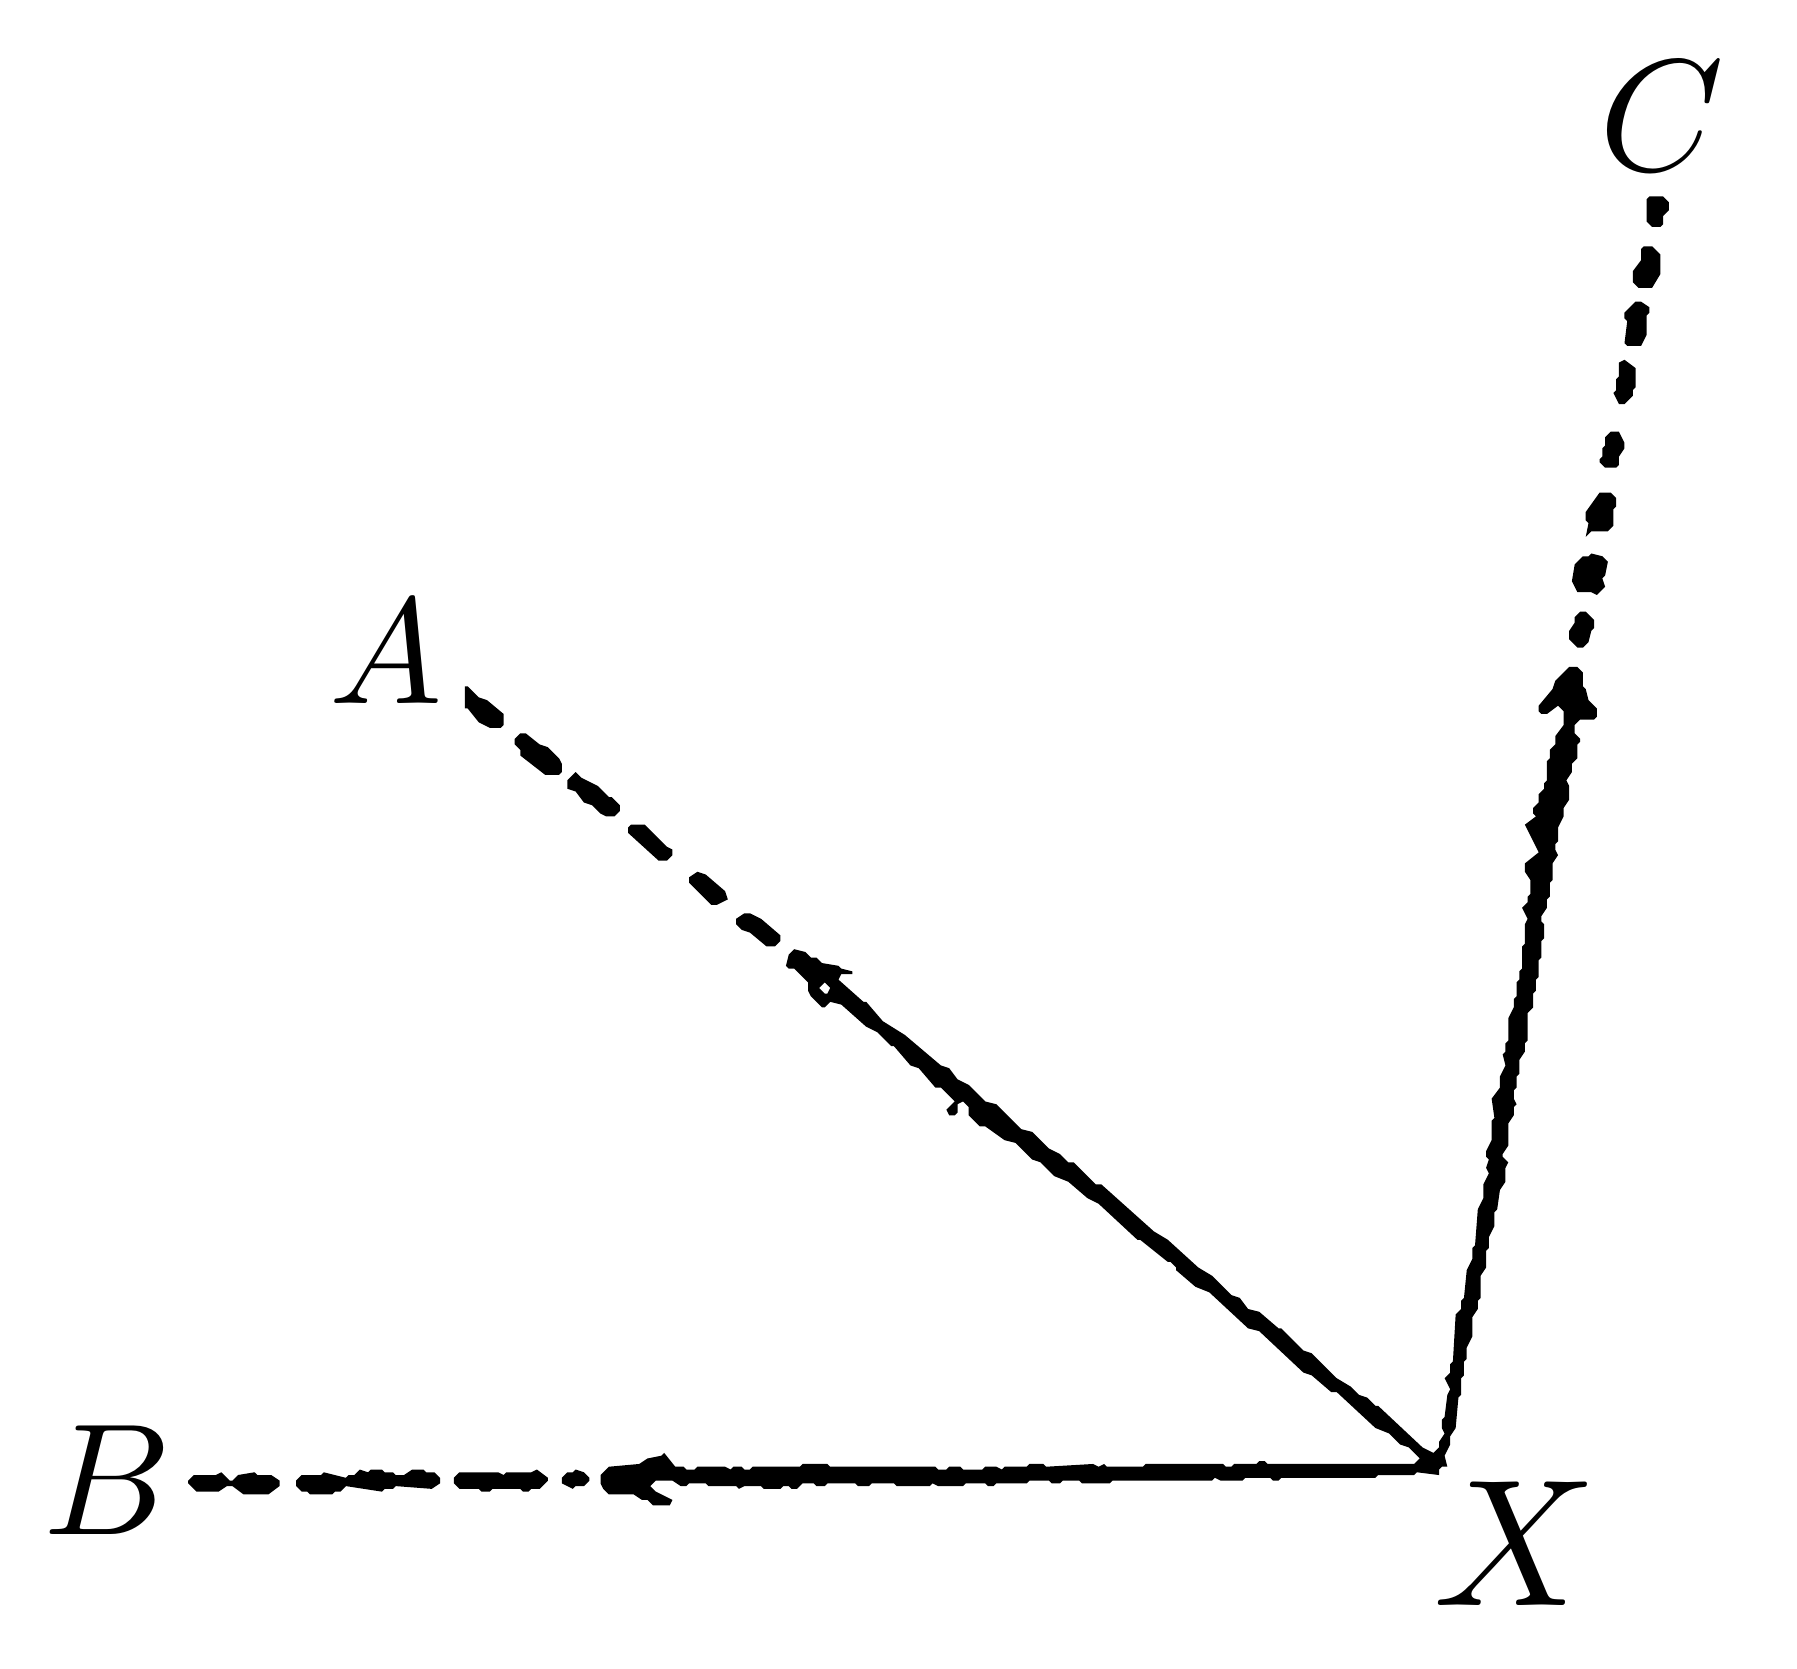
\begin{tikzpicture}[x=1pt,y=-1pt]
\path[use as bounding box] (0,0) rectangle (629,583);
\path[fill=black,draw=none,even odd rule]
(58,525) -- (58,526) -- (61,529) -- (69,529) -- (72,527) -- (74,527) -- (78,530) -- (87,530) -- (91,527) -- (91,525) -- (88,523) -- (83,523) -- (82,522) -- (76,523) -- (74,525) -- (73,525) -- (70,522) -- (68,523) -- (60,523) -- cycle
(203,524) -- (201,522) -- (198,521) -- (197,522) -- (195,522) -- (193,524) -- (193,526) -- (197,528) -- (198,527) -- (201,527) -- (203,525) -- cycle
(188,524) -- (184,521) -- (182,522) -- (173,522) -- (172,523) -- (170,522) -- (156,522) -- (154,524) -- (154,526) -- (156,528) -- (163,528) -- (164,529) -- (167,529) -- (168,528) -- (178,528) -- (179,529) -- (181,529) -- (182,528) -- (185,528) -- (188,525) -- cycle
(97,525) -- (97,527) -- (99,529) -- (101,529) -- (102,530) -- (110,530) -- (111,529) -- (113,529) -- (115,527) -- (128,529) -- (129,528) -- (132,528) -- (133,527) -- (146,528) -- (149,526) -- (149,524) -- (147,522) -- (144,522) -- (143,521) -- (139,521) -- (136,523) -- (133,523) -- (132,522) -- (129,522) -- (128,521) -- (124,521) -- (123,522) -- (120,521) -- (118,523) -- (116,523) -- (115,524) -- (107,522) -- (106,523) -- (99,523) -- cycle
(256,322) -- (256,324) -- (258,326) -- (261,327) -- (267,332) -- (270,332) -- (272,330) -- (272,328) -- (265,322) -- (261,320) -- (259,320) -- cycle
(239,307) -- (239,309) -- (247,317) -- (249,317) -- (253,315) -- (252,312) -- (245,306) -- (242,305) -- cycle
(217,289) -- (217,291) -- (228,301) -- (231,301) -- (233,299) -- (233,297) -- (231,296) -- (223,288) -- (218,288) -- cycle
(195,272) -- (195,275) -- (198,276) -- (201,280) -- (204,281) -- (207,284) -- (209,285) -- (212,285) -- (214,283) -- (214,281) -- (211,278) -- (210,278) -- (206,274) -- (200,271) -- (198,269) -- cycle
(176,257) -- (176,259) -- (178,261) -- (178,263) -- (187,270) -- (192,270) -- (193,269) -- (193,266) -- (192,264) -- (188,260) -- (185,259) -- (180,255) -- (178,255) -- cycle
(158,238) -- (158,246) -- (159,246) -- (163,251) -- (167,253) -- (171,253) -- (172,252) -- (172,248) -- (166,243) -- (163,242) -- (159,238) -- cycle
(562,233) -- (560,231) -- (557,231) -- (552,236) -- (551,239) -- (546,245) -- (546,247) -- (547,248) -- (549,248) -- (553,245) -- (555,247) -- (555,252) -- (552,256) -- (552,259) -- (550,261) -- (550,264) -- (549,265) -- (549,272) -- (548,273) -- (548,275) -- (546,277) -- (546,280) -- (544,282) -- (544,284) -- (545,285) -- (541,288) -- (546,298) -- (541,302) -- (541,305) -- (543,308) -- (543,313) -- (542,314) -- (542,316) -- (540,318) -- (542,322) -- (541,324) -- (541,331) -- (540,332) -- (540,340) -- (539,341) -- (539,344) -- (538,345) -- (538,350) -- (537,351) -- (537,354) -- (535,358) -- (535,366) -- (534,367) -- (534,370) -- (533,371) -- (534,375) -- (532,379) -- (532,383) -- (529,387) -- (530,394) -- (529,395) -- (529,402) -- (527,406) -- (527,408) -- (528,409) -- (527,412) -- (528,414) -- (526,418) -- (526,423) -- (524,427) -- (523,440) -- (522,441) -- (522,445) -- (520,449) -- (519,459) -- (518,460) -- (518,463) -- (516,465) -- (515,482) -- (514,483) -- (514,486) -- (512,488) -- (514,492) -- (513,494) -- (512,502) -- (511,503) -- (511,506) -- (512,508) -- (510,511) -- (510,513) -- (508,515) -- (504,513) -- (488,498) -- (487,498) -- (484,495) -- (481,494) -- (478,491) -- (473,488) -- (464,479) -- (461,478) -- (453,470) -- (452,470) -- (445,464) -- (441,463) -- (438,459) -- (435,458) -- (428,451) -- (423,448) -- (412,438) -- (407,435) -- (388,418) -- (386,418) -- (378,410) -- (376,410) -- (373,407) -- (369,405) -- (363,399) -- (359,398) -- (350,389) -- (346,388) -- (340,382) -- (336,380) -- (333,376) -- (330,375) -- (317,364) -- (309,359) -- (303,352) -- (302,352) -- (293,344) -- (294,342) -- (298,342) -- (298,341) -- (294,340) -- (293,339) -- (287,338) -- (285,336) -- (283,336) -- (281,334) -- (277,333) -- (275,335) -- (274,339) -- (275,340) -- (277,340) -- (282,345) -- (282,348) -- (283,350) -- (287,354) -- (288,354) -- (290,352) -- (294,353) -- (303,361) -- (307,363) -- (312,368) -- (313,368) -- (319,375) -- (322,376) -- (328,383) -- (330,383) -- (335,388) -- (332,391) -- (333,393) -- (335,393) -- (336,392) -- (336,389) -- (338,388) -- (340,390) -- (340,393) -- (344,397) -- (346,397) -- (353,402) -- (357,403) -- (363,409) -- (366,410) -- (371,415) -- (376,417) -- (383,423) -- (387,425) -- (401,438) -- (402,438) -- (412,446) -- (413,446) -- (415,448) -- (415,449) -- (422,455) -- (427,457) -- (441,470) -- (445,471) -- (461,486) -- (464,487) -- (471,493) -- (473,493) -- (487,506) -- (492,508) -- (496,512) -- (499,513) -- (503,517) -- (501,519) -- (448,519) -- (447,518) -- (445,518) -- (444,519) -- (436,519) -- (435,520) -- (433,520) -- (432,519) -- (404,519) -- (403,520) -- (390,520) -- (389,519) -- (387,520) -- (385,519) -- (368,520) -- (367,519) -- (362,519) -- (361,520) -- (353,520) -- (352,521) -- (350,520) -- (346,520) -- (345,521) -- (338,521) -- (337,520) -- (333,520) -- (332,521) -- (329,521) -- (328,520) -- (290,520) -- (289,519) -- (280,519) -- (279,520) -- (262,520) -- (261,521) -- (259,521) -- (258,520) -- (255,520) -- (254,521) -- (252,520) -- (242,520) -- (241,521) -- (238,521) -- (237,520) -- (234,520) -- (230,515) -- (229,516) -- (224,517) -- (221,519) -- (210,520) -- (207,523) -- (207,526) -- (208,528) -- (210,530) -- (219,530) -- (222,532) -- (224,532) -- (226,534) -- (232,534) -- (233,532) -- (227,529) -- (225,527) -- (227,525) -- (233,525) -- (236,527) -- (238,527) -- (239,526) -- (245,526) -- (246,527) -- (256,527) -- (257,528) -- (259,527) -- (265,527) -- (266,528) -- (272,528) -- (273,527) -- (275,527) -- (276,528) -- (278,528) -- (280,526) -- (284,526) -- (285,527) -- (288,527) -- (289,526) -- (299,526) -- (300,527) -- (304,527) -- (305,526) -- (313,526) -- (314,527) -- (326,527) -- (327,526) -- (329,527) -- (338,527) -- (339,526) -- (346,526) -- (347,527) -- (349,527) -- (350,526) -- (361,526) -- (362,525) -- (369,525) -- (370,526) -- (373,526) -- (374,525) -- (380,525) -- (381,526) -- (391,526) -- (392,525) -- (428,525) -- (429,524) -- (431,525) -- (439,525) -- (440,524) -- (449,524) -- (450,525) -- (452,525) -- (453,524) -- (487,524) -- (488,523) -- (501,523) -- (502,522) -- (510,523) -- (510,521) -- (511,520) -- (513,520) -- (512,516) -- (514,512) -- (514,509) -- (516,506) -- (517,495) -- (518,494) -- (518,488) -- (519,487) -- (519,482) -- (520,481) -- (520,477) -- (522,473) -- (522,466) -- (524,463) -- (524,460) -- (525,459) -- (525,451) -- (527,448) -- (527,442) -- (528,441) -- (528,437) -- (530,433) -- (530,428) -- (531,427) -- (532,420) -- (534,417) -- (534,412) -- (535,410) -- (533,408) -- (533,407) -- (535,404) -- (535,396) -- (537,393) -- (537,390) -- (538,389) -- (537,387) -- (537,384) -- (538,383) -- (538,379) -- (539,378) -- (539,373) -- (541,370) -- (541,367) -- (542,366) -- (542,356) -- (544,354) -- (544,349) -- (545,348) -- (545,344) -- (546,343) -- (546,337) -- (547,336) -- (547,330) -- (548,329) -- (548,324) -- (547,323) -- (547,321) -- (549,318) -- (549,315) -- (550,314) -- (550,309) -- (551,308) -- (551,302) -- (553,299) -- (552,297) -- (552,295) -- (553,294) -- (553,289) -- (555,285) -- (555,282) -- (557,279) -- (557,274) -- (556,272) -- (558,269) -- (558,266) -- (560,264) -- (560,259) -- (561,258) -- (561,257) -- (559,255) -- (559,252) -- (561,250) -- (566,250) -- (567,249) -- (567,246) -- (564,243) -- (563,239) -- (562,238) -- cycle
(288,345) -- (290,347) -- (289,349) -- (288,349) -- (286,347) -- cycle
(563,211) -- (561,211) -- (559,213) -- (559,215) -- (557,218) -- (557,221) -- (560,224) -- (562,224) -- (564,222) -- (565,218) -- (566,217) -- (566,214) -- cycle
(565,190) -- (564,191) -- (562,191) -- (559,194) -- (558,200) -- (560,204) -- (565,204) -- (567,205) -- (570,202) -- (569,199) -- (570,198) -- (571,193) -- (569,191) -- cycle
(572,168) -- (568,168) -- (563,175) -- (563,178) -- (564,179) -- (563,184) -- (565,182) -- (571,182) -- (573,180) -- (573,174) -- (574,173) -- (574,170) -- cycle
(575,146) -- (572,146) -- (570,148) -- (570,151) -- (569,152) -- (569,155) -- (568,156) -- (568,157) -- (570,159) -- (574,159) -- (575,158) -- (575,155) -- (577,152) -- (577,150) -- cycle
(577,120) -- (575,121) -- (575,126) -- (574,127) -- (574,131) -- (573,132) -- (575,136) -- (577,136) -- (580,133) -- (580,131) -- (581,130) -- (581,123) -- cycle
(583,99) -- (581,99) -- (577,103) -- (577,105) -- (578,106) -- (577,114) -- (578,115) -- (583,115) -- (585,111) -- (585,104) -- (586,103) -- (586,101) -- cycle
(584,79) -- (583,80) -- (583,84) -- (580,88) -- (580,92) -- (582,94) -- (587,94) -- (590,89) -- (590,82) -- (587,79) -- cycle
(586,61) -- (585,62) -- (585,70) -- (587,72) -- (590,72) -- (591,71) -- (591,68) -- (593,66) -- (593,63) -- (591,61) -- cycle;
\node[inner sep=0pt,font=\fontsize{10}{10}\selectfont] at (590.5,32.0) {\scalebox{5.742}{$C$}};
\node[inner sep=0pt,font=\fontsize{10}{10}\selectfont] at (129.5,225.5) {\scalebox{5.445}{$A$}};
\node[inner sep=0pt,font=\fontsize{10}{10}\selectfont] at (29.0,525.0) {\scalebox{5.742}{$B$}};
\node[inner sep=0pt,font=\fontsize{10}{10}\selectfont] at (537.5,548.0) {\scalebox{6.534}{$X$}};
\end{tikzpicture}%
}
\end{center}
